\documentclass[11pt]{article}
\usepackage[utf8]{inputenc}
\usepackage[rightcaption]{sidecap}
\usepackage{float}
\usepackage{wrapfig}
\usepackage{natbib}
\usepackage{algorithm}% http://ctan.org/pkg/algorithm
\usepackage{algpseudocode}% http://ctan.org/pkg/algorithmicx
\usepackage{graphicx}
\usepackage{caption}
\usepackage{capt-of}
\usepackage{subcaption}
\usepackage{verbatim}
\usepackage{grffile}
\usepackage[subsection]{placeins}
\usepackage{geometry}
\usepackage[framed ,numbered]{matlab-prettifier}

\geometry{
 a4paper,
 left=25mm,
 top=20mm,
 right = 20 mm
 } 

%\floatstyle{boxed} % or whatever
%\restylefloat{figure}
\graphicspath{ {./images/} }
\newcommand{\snr}{$E_{b}/N_{0}$}
\renewcommand{\baselinestretch}{1} 

\begin{document}

\begin{titlepage}

\newcommand{\HRule}{\rule{\linewidth}{0.9mm}} % Defines a new command for the horizontal lines, change thickness here

\center % Center everything on the page
%\\[0.5cm]
%----------------------------------------------------------------------------------------
%    HEADING SECTIONS
%----------------------------------------------------------------------------------------

\textsc{\Large \textbf{Department of Electronic and Telecommunication
Engineering}\small \\EN 4053 - Digital Communication II}\\[10mm] % Name of your university/college

%----------------------------------------------------------------------------------------
%    LOGO SECTION
%----------------------------------------------------------------------------------------

\includegraphics[ height=5cm]{uomlogo.png}\\[0.1cm]
\textsc{\Large  \textbf{University Of Moratuwa}}\\[0.5cm] 
%----------------------------------------------------------------------------------------
\textsc{\large \\Assignment 2}\\[0cm] % Minor heading such as course title

%----------------------------------------------------------------------------------------
%    TITLE SECTION
%----------------------------------------------------------------------------------------

%\HRule
%\\[1cm]
{ \huge \bfseries Error Correction Coding}\\[9cm] % Title of your document
%\HRule 
%\\[1cm]
 
%----------------------------------------------------------------------------------------
%    AUTHOR SECTION
%----------------------------------------------------------------------------------------


\emph{\large \textbf{Group Members:}}\\
\begin{tabular}{ll}\large
\large A. L. A. V. \textsc{Isuru}& \large - 140239D\\
\large H.D. \textsc{Fernando}& \large - 140154L\\
\large W.D.A.P. \textsc{Ravinath}& \large - 140530L
\end{tabular}\\[1cm]




% If you don't want a supervisor, uncomment the two lines below and remove the section above
%\Large \emph{Author:}\\
%John \textsc{Smith}\\[3cm] % Your name

%----------------------------------------------------------------------------------------
%    DATE SECTION
%----------------------------------------------------------------------------------------

{\large \today}\\[0.1cm] % Date, change the \today to a set date if you want to be precise



\vfill % Fill the rest of the page with whitespace

\end{titlepage}

\clearpage

%----------------------------------------------------------------------------------------%
%                                     VIJITHA                                            %
%----------------------------------------------------------------------------------------%



\section{Transmission of data over an AWGN channel}
\subsection{Implement the baseband communication system shown in Figure 1 in Matlab}
\begin{center}
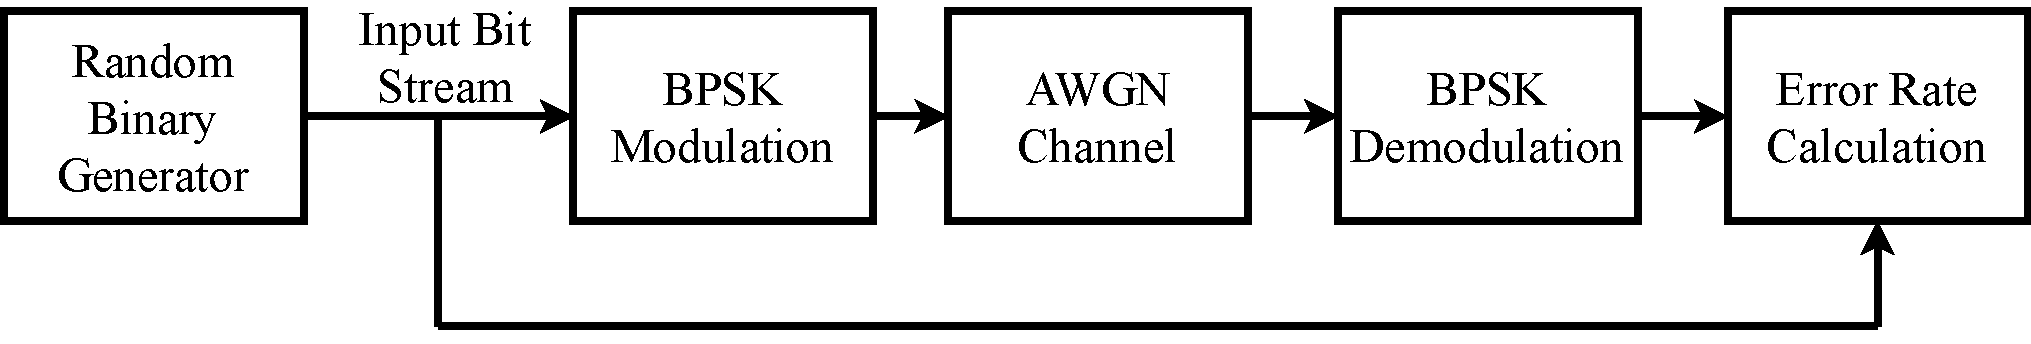
\includegraphics[width=.7\textwidth]{baseband-com-in-awgn-ch.pdf}
\label{fig:baseband-com-sys}
\captionof{figure}{Baseband Communication System in an AWGN Channel}
\end{center}

\lstinputlisting[style=Matlab-editor, caption={Calculating error amount per one iteration}]{UNCODED_SYSTEM.m}
\lstinputlisting[style=Matlab-editor, caption={Average error count per one signal}]{BER.m}

\subsection{Transmit powers corresponding to different Eb/No values given in Table 1.}

\begin{table}[h]
\centering
\caption{\label{tab:transmit_power_levels}Transmit power levels to achieve different $E_{b}/N_{0}$.}
\begin{tabular}{|c|c|c|c|c|c|c|c|c|c|}

\hline
$E_{b}/N_{0}$ (dB) & -4 & -2 & 0 & 2 & 4 & 6 & 8 & 10 & 12 \\\hline
$P_{\tau}$ (W) & 0.0796 & 0.1262 & 0.2000 & 0.3170 & 0.5024 &	0.7962 &	1.2619	& 2.0000 & 3.1698 \\\hline             % ***** EDIT HERE *****

\end{tabular}

\end{table}

\subsection{Simulations}
\subsection{Obtain the average bit error rate (BER) for each Eb/No value.}
\lstinputlisting[style=Matlab-editor, caption={Calculating BER}]{BER_for_table.m}


\begin{table}[h]
\centering
\caption{BER for corresponding $E_{b}/N_{0}$ values}
\begin{tabular}{|c|c|c|c|c|c|c|c|c|c|}

\hline
\snr (dB) & -4     &     -2 &      0 &      2 &      4 &         6 &          8 &     10 &     12 \\\hline
$BER$     & 0.0796 & 0.1262 & 0.2000 & 0.3170 & 0.5024 &	0.7962 &	1.2619	& 2.0000 & 3.1698 \\\hline

\end{tabular}

\end{table}

%----------------------------------------------------------------------------------------%
%                                     HESHAN                                             %
%----------------------------------------------------------------------------------------%
\section{Error correction using Hamming codes}
\subsection{Table 1's answer}
Answer
\subsection{Table 1's answer}
Answer
\subsection{Table 1's answer}
Answer
\subsection{Table 1's answer}
Answer
\subsection{Table 1's answer}
Answer

%----------------------------------------------------------------------------------------%
%                                     AMILA                                              %
%----------------------------------------------------------------------------------------%

\section{Error correction using Convolution codes}
\subsection{Simulink Model}
\begin{center}
    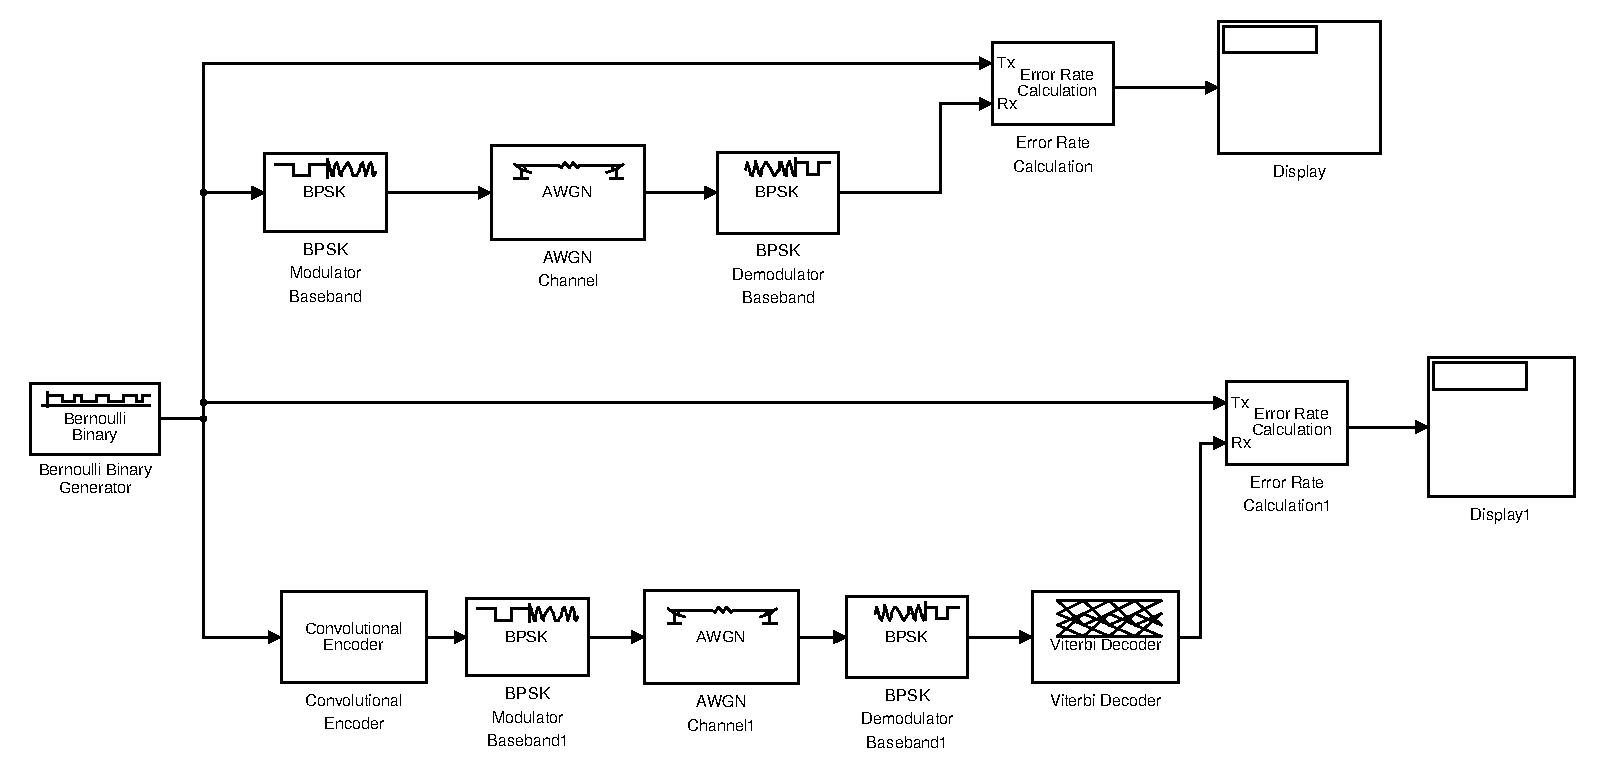
\includegraphics[width=.8\textwidth]{q6-model.pdf}
    \label{fig:q6-model}
    \captionof{figure}{Baseband communication system with Convolution coder / Viterbi decoder in an AWGN channel \cite{simulink}}
\end{center}

\subsection{Effect of Convolution coding to BER}
\begin{table}[h]
    \centering
    \caption{\label{tab:transmit_power_levels_sim}BER for Convolutional and Uncoded systems with respect to $E_{b}/N_{0}$ value.}
    \begin{tabular}{|c|c|c|c|c|c|c|c|c|c|}
        \hline
        \snr (dB) & -4       & -2       & 0         & 2         & 4       & 6        & 8         & 10 & 12 \\\hline
        Uncoded   & 0.1789   & 0.1296   & 0.07894   & 0.03753   & 0.01269 & 0.002377 & 0.0002126 & 0  & 0 \\\hline
        Coded     & 0.4195   & 0.2695   & 0.04295   & 0.0006221 & 0       & 0        & 0         & 0  & 0 \\\hline
    \end{tabular}
\end{table}

\subsection{BER Graph}
\begin{center}
    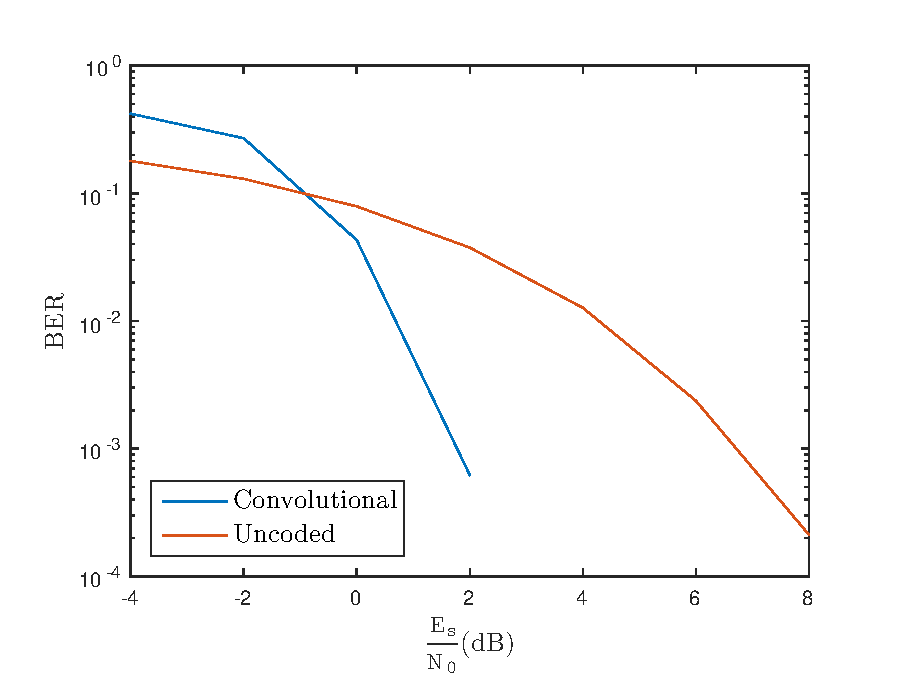
\includegraphics[width=.5\textwidth]{q613.eps}
    \label{fig:q613}
    \captionof{figure}{BER Uncoded Vs. Convolutional Coded}
\end{center}

%----------------------------------------------------------------------------------------%
%                                     DISCUSSION                                         %
%----------------------------------------------------------------------------------------%

\section{Discussion}
\subsection{Comment on and explain the BER plots you have obtained for Uncoded, Hamming coded and
convolution coded systems}
Answer
\subsection{Briefly explain the factors required to be taken into consideration in selecting a suitable
channel coding scheme for a given application}
Answer
\bibliographystyle{plain}
\bibliography{references}
\end{document}

 
